\chapter{Basic Analog Circuits}
In this chapter, we will see how non-linear elements are used in electrical circuits. We discuss the concept of a load line, both static and dynamic, and study the small-signal response of a non-linear element, which essentially requires a linearization around an operating point. Finally, we provide small-signal models for both diodes and transistors at high and low frequencies.

\section{Non-linear elements in circuits}
\label{sec:nonlin_circuits}
In this section, we will see how non-linear elements like diodes and transistors are used in electrical circuits. In principle, adding a non-linear element makes the analysis of the circuit a lot harder, compared to circuits with only linear elements (resistors, capacitors, inductors, \ldots). In practice however, we will rely on a graphical solution method, which simplifies the analysis while still being rigorous.
\subsection{The Diode as a Circuit Element}
Let's use a diode as a lumped element in an electronic circuit, as in the  figure below. 

\begin{wrapfigure}{r}{3.5cm}
	\centering
	\includegraphics[width=3cm]{figures/ch02/diode1.jpg}
	\caption{}
	\label{fig:diode1}
\end{wrapfigure}
By applying KVL, we obtain the equation of the \textbf{load-line}:
$$
E - v_D = R \; i_D
$$
This equation has to be combined with the diode I-V characteristic:
$$
i_D = \phi(v_D) = I_S (e^{v_D/v_{th}} - 1)
$$
Form a formal point of view, we have two unknowns, $v_D$ and $i_d$, and two equations, so in principle we can solve for both unknowns. However, there is no analytical solution to our problem, so we prefer a graphical method.\\
In figure \ref{fig:diode2} we combine $i_D = \phi(v_D)$ (the red curve) with the expression of the load line (green line).

\begin{figure}[h!]
	\centering
	\includegraphics[width=12cm]{figures/ch02/diode2.jpg}
	\caption{I-V with load line (a) with $E > 0.6 V$ and (b) $E < 0.6$ V}
	\label{fig:diode2}
\end{figure}
We apply a simplification and assume that $v_D = V_{DQ} \approx 0.6$ V. The operating point\footnote{The letter $Q$ stands for \emph{quiescent}} $Q$ lies at the intersection of both lines. In order for the diode to conduct, we can immediately conclude by comparing both figures that it is necessary that $E > 0.6V = V_{DQ}$. The diode current is easily calculated as
$$
i_D \approx I_{DQ} = \frac{E - V_{DQ}}{R}
$$
We can conclude that the diode will always conduct as long as $E > 0.6$ V. Variations in $E$ only mean that the load line will move parallel. The operating point $(V_{DQ},  I_{DQ})$ can only move vertically because of the nature of $\phi(v_D)$ when $v_D > 0.6$ V. Only when $E$ becomes smaller than $0.6$ V will conduction stop until we reach the Zener region. Remember that the $0.6$ V is specific for silicon.\\

\begin{minipage}{.6\textwidth}
	As an example, consider the circuit in figure \ref{fig:diode3}. It is not obvious when the diode will conduct, so let's replace the current source and the resistor by the Thevenin equivalent, namely a resistor $R_{th} = R$ and a voltage source $V_{th} = R I_0$ in \textbf{series} with this resistor. This circuit is identical to the one in figure \ref{fig:diode1} with a load line through the points $(R\;I_0, 0)$ and $(0, I_0)$. We can conclude that the transistor will conduct when $V_{th} = R\;I_0 > 0.6$ V. Furthermore, when $R\rightarrow \infty$ and the resistor become an open circuit, the load line will become a horizontal line through $I_0$.
\end{minipage}
\begin{minipage}{.5\textwidth}
	\centering
	\includegraphics[width=5cm]{figures/ch02/diode3.jpg}
	\captionof{figure}{With current source}
	\label{fig:diode3}
\end{minipage}%

\subsection{The BJT as a Circuit Element}
A typical bipolar transistor circuit is shown in figure \ref{fig:bjt_load1}(b). To analyze this circuit, we cut at the entrance of the base and replace the left loop of resistors $R_1$ and $R_2$ and the supply voltage $E$ by the Thevenin equivalent circuit in figure  \ref{fig:bjt_load1}(a).

\begin{figure}[h!]
	\centering
	\includegraphics[width=12cm]{figures/ch02/bjt_load1.jpg}
	\caption{(a) Transistor circuit and (b) simplified with Thevenin} 
	\label{fig:bjt_load1}
\end{figure}
The Thevenin voltage $E_B$ and impedance $R_B$ are easily computed by seeing that (a) the voltage at the base is the result of applying a voltage divider to the supply voltage $E$, and (b) that when we ground $E$ (as required by the Thevenin rules) $R_1$ and $R_2$ are in parallel:
\begin{equation}
	\begin{split}
		E_B &= \frac{R_2}{R_1 + R_2} E \\
		R_B &= R_1 || R_2 = \frac{R_1 R_2}{R_1 + R_2}
	\end{split}
\end{equation}
In this left loop, we can write:
\begin{equation}
	\begin{split}
		E_B - v_{BE} &= R_B \; i_B \\
		%E - v_{CE} &= R_C \; i_C
	\end{split}
\end{equation}
Consider the right loop, which consists of resistor $R_C$ and the voltage $v_{CE}$. In this loop, we can write:
\begin{equation}
	\begin{split}
		%E_B - v_{BE} &= R_B \; i_B \\
		E - v_{CE} &= R_C \; i_C
	\end{split}
\end{equation}
Let's assume that all the currents are constant and we have biased the transistor in its operating point. We indicate this by adding a $Q$ to the currents and voltages, just as for the diode. With this convention, we can rewrite these equations to obtain:
\begin{equation}
	\begin{split}
		I_{BQ} &= \frac{E_B - V_{BEQ}}{R_B}\\
		V_{CEQ} &= E - R_C \; I_{CQ}
	\end{split}
\end{equation}
with $V_{BEQ} \approx 0.6$ V because we want to bias the base-emitter junction in the forward (conducting) region. From the diode analysis, we know this will be the case when $E_B > 0.6$ V. We also know the relation between $I_{BQ}$ and $I_{CQ}$ (neglecting any leak currents):
\begin{equation}
	\begin{split}
		I_{CQ} &= \beta \; I_{BQ}
	\end{split}
\end{equation}
where $\beta$ is given by the manufacturer and is typically very high, but it can vary a lot from one transistor to the next. With this equation, we have enough information to compute all currents and voltages:
\begin{enumerate}
	\item We know $R_B$ and $E_B$, and we assume $V_{BEQ} = 0.6$ V, so we can compute $I_{BQ}$.
	\item We know $\beta$, so we can compute $I_{CQ}$.
	\item We can now compute $V_{CE}$.
\end{enumerate}
All these calculations can all be represented graphically; see the (idealized) BJT characteristic in figure \ref{fig:bjt_load2}.
\begin{figure}[h!]
	\centering
	\includegraphics[width=12cm]{figures/ch02/bjt_load2.jpg}
	\caption{(a) Transistor circuit and (b) simplified with Thevenin} 
	\label{fig:bjt_load2}
\end{figure}
The figure on the left represents the left loop, with the load line $E_B - v_{BE} = R_B \; i_B $ in green and the $v_{BE}$ junction characteristic in red. The intersection between both functions is the operating point $Q = (V_{BEQ}, I_{BQ})$.\\
The right loop is shown in the graph on the right; the horizontal line on which the transistor operates is given by $I_{C} = \beta \; I_{B}$ and the load line is given by $V_{CE} = E - R_C \; I_{C}$. Once again, the operating point is there where both lines intersect.\\
We can reason about the operation of the circuit by thinking about these figures. For example, if $R_B$ would decrease, the slope of the $I_B - V_{BE}$ load-line would increase, so that the operating point $Q$ will move up and $I_{BQ}$ will increase. This increase will cause in increase of $I_{CQ}$ in the graph on the right, and the operating point will move along the load line to a higher $I_{C}$ and a lower $V_{CE}$.\\
We can conclude that:
\begin{itemize}
	\item The left loop determines $I_{BQ}$.
	\item By assumption, we are in the normal working domain and $I_{CQ} = \beta I_{BQ}$.
	\item The right loop gives  $V_{CEQ}$.
	\item Given $Q = (V_{CEQ}, \; I_{CQ})$, we verify we are in the normal working domain.
\end{itemize}
Let's discuss a couple of edge cases:
\begin{itemize}
	\item If $E_{B} < 0.6$ V then $V_{BEQ} < 0.6$ V. Then $I_{BQ} \approx 0$ and $I_{CQ} \approx 0$ (neglecting leakage current). See figure \ref{fig:bjt_load3}(a). If that's the case, the operating point is $Q = (V_{CEQ} = E, 0)$ and the transistor is blocked (\emph{cut-off mode}). 
	\begin{figure}[h!]
		\centering
		\includegraphics[width=14cm]{figures/ch02/bjt_load3.jpg}
		\caption{(a) $V_{BEQ} < 0.6$V and (b) $V_{CEQ} \approx V_{CE, Sat}$} 
		\label{fig:bjt_load3}
	\end{figure}
	\item As $V_{BEQ}$ and $I_{BQ}$ keep increasing, $I_{CQ}$ will become larger and eventually $V_{CEQ}$ will become too small to keep the transistor in active mode. Then $I_{CQ} \ne \beta \;I_{BQ}$ and $V_{CEQ} \approx V_{CE, Sat}$. So, in that case, $I_{CQ} = \frac{E-V_{CE,Sat}}{R_C}$. The transistor is \emph{saturated}.
\end{itemize}
\subsection{The MOSFET as a Circuit Element}
Just as for the BJT, we consider a biasing circuit for the n-channel MOSFET transistor as in figure \ref{fig:mos_load1}(a) and we simplify the circuit with a Thevenin equivalent circuit - like we did before - as in figure \ref{fig:mos_load1}(b).
\begin{figure}[h!]
	\centering
	\includegraphics[width=10cm]{figures/ch02/mos_load1.jpg}
	\caption{(a) MOS Transistor circuit and (b) simplified with Thevenin} 
	\label{fig:mos_load1}
\end{figure}
with 
\begin{equation}
	\begin{split}
		E_B-G &= \frac{R_2}{R_1 + R_2} E \\
		R_G &= R_1 || R_2 = \frac{R_1 R_2}{R_1 + R_2}
	\end{split}
\end{equation}
Note that the gate current $I_G = 0$ as the gate is a capacitor where the DC current is zero. And just as for the BJT, we can express an equation for the left and right loop:
\begin{equation}
	\begin{split}
		V_{GSQ} &= E_G \text{ because } I_{G} = 0\\
		I_{DSQ} &= \frac{\mu_n C_{ox}}{2} \frac{W}{L} (V_{GSQ} - V_T)^2 \text{ if } V_{GSQ} > V_T\\
		V_{DSQ} &= E - R_D \; I_{DSQ} \text{ if } V_{DSQ} > V_{GSQ} - V_T
	\end{split}
\end{equation}
 The last condition is required for the transistor to be saturated, which is similar to the active mode for a BJT.\\
 We can also represent these equations graphically. Figure \ref{fig:mos_load2}(a) represents the quadratic relation between $I_{DS}$ and $V_{GS}$ to determine $V_{GSQ}$. As long as $V_{DS} > V_{GSQ} - V_T$, figure \ref{fig:mos_load2}(b) gives the value of $V_{DSQ}$.
 \begin{figure}[h!]
 	\centering
 	\includegraphics[width=14cm]{figures/ch02/mos_load2.jpg}
 	\caption{(a) $i_{DS} = f(v_{DS})$ and (b) $I_{DS} = f(V_{DS})$}
 	\label{fig:mos_load2}
 \end{figure}


 \subsection{Additional remarks}
 For both type of transistors, there are three working domains, as in figure \ref{fig:transistor_overview}:
 \begin{itemize}
 	\item MOSFET: blocked, saturated, linear
 	\item BJT: blocked, normal (or active), saturated
 \end{itemize}
\begin{figure}[h!]
	\centering
	\includegraphics[width=12cm]{figures/ch02/overview.jpg}
	\caption{(a) $i_{DS} = f(v_{DS})$ and (b) $I_{DS} = f(V_{DS})$}
	\label{fig:transistor_overview}
\end{figure}
\subsection{A more general circuit}
\label{sec:general_circuit}
To improve the linearity (see the chapter on feedback) and biasing of the circuit, an emitter resistance $R_E$ is often added, as in figure \ref{fig:general1a}. Just as before, the left side is simplified with the Thevenin equivalent (see \ref{fig:general1b}).

\begin{figure}[h!]
	\centering
	\begin{minipage}{.5\textwidth}
		\centering
		\includegraphics[width=4cm]{figures/ch02/general1a.jpg}
		\captionof{figure}{General circuit}
		\label{fig:general1a}
	\end{minipage}%
	\begin{minipage}{.5\textwidth}
		\centering
		\includegraphics[width=5cm]{figures/ch02/general1b.jpg}
		\captionof{figure}{Thevenin simplification}
		\label{fig:general1b}
	\end{minipage}
	%	\label{fig:explore}
\end{figure}
Once again, we can write the KVL in left and right loop:
\begin{equation}
	\begin{split}
		E_B - V_{BEQ} &= R_B I_{BQ} + R_E I_{EQ} = R_B I_{BQ} + R_E (\beta + 1) I_{BQ} \\
		E_B - V_{BEQ} &= R_B \frac{I_{CQ}}{\beta} + R_E (\beta + 1) \frac{I_{CQ}}{\beta} \approx \frac{R_B}{\beta} I_{CQ} + R_E I_{EQ}
	\end{split}
\end{equation}
where we have used $I_{CQ} = \beta I_{BQ}$ because we suppose we're working in the normal operating region. These equations lead to expressions for current $I_{CQ}$ and voltage $V_{CEQ}$:
\begin{equation}
	\begin{split}
		I_{CQ} &= \frac{E_B - V_{BEQ}}{\frac{R_B}{\beta} + R_E}\\
		V_{CEQ} &= E - (R_C + R_E) I_{CQ}
	\end{split}
	\label{eq:four_resitors1}
\end{equation}
They can be plotted on the different I-V characteristics as in figure \ref{fig:general2}. Notice that the figure on the left gives $i_C$ as function of $v_{BE}$. Since the relation between $i_B$ and $v_{BE}$ is the exponential diode characteristic, the same goes goes for the relation between $i_C = \beta i_B$ and $v_{BE}$.
\begin{figure}[h!]
	\centering
	\includegraphics[width=12cm]{figures/ch02/general2.jpg}
	\caption{(a) Load line: $I_{CQ} = \frac{E_B - V_{BEQ}}{\frac{R_B}{\beta} + R_E}$ (b) $V_{CEQ} = E - (R_C + R_E) I_{CQ}$}
	\label{fig:general2}
\end{figure}

We can apply the same reasoning to the $4$-resistor MOSFET circuit form figure \ref{fig:mos_load3}, for which we also can simplify the left loop with the Thévenin equivalent of figure \ref{fig:mos_load4}.
\begin{figure}[h!]
	\centering
	\begin{minipage}{.5\textwidth}
		\centering
		\includegraphics[width=5cm]{figures/ch02/mos_load3.jpg}
		\captionof{figure}{}
		\label{fig:mos_load3}
	\end{minipage}%
	\begin{minipage}{.5\textwidth}
		\centering
		\includegraphics[width=6cm]{figures/ch02/mos_load4.jpg}
		\captionof{figure}{}
		\label{fig:mos_load4}
	\end{minipage}
	%	\label{fig:explore}
\end{figure}
The operating  point $Q$ is determined by:
\begin{align*}
	&\text{The equation of the left loop: } E_G - V_{GSQ} = R_S I_{DSQ} \\
	&\text{The transistor characteristic: } I_{DSQ} = \frac{K}{2}\frac{W}{L} (V_{GSQ} - V_T)^2 \\
	&\text{The equation of the right loop: } V_{DSQ} = E - (R_D + R_S)I_{DSQ}
\end{align*}
To find $V_{GSQ}$ and $I_{DSQ}$, use the first two equations; only one root is valid for $V_{GSQ}$. $V_{DSQ}$ follows immediately from the third equation.
\section{Small-Signal Response}
\label{sec:small_signal_response}
In this section, we will introduce the concept of a small-signal response, namely how do voltage and currents in a circuit change when we apply only a small change to the input values. The general idea is that we design the circuit such that it operates at an operating point $Q$, and we linearize the circuit around this operating point to study only small deviations. We will use the diode as an example. in section \ref{sec:small_signal_model} we apply the same reasoning to transistors.\\
First, we introduce some notation to distinguish large-signal from small signal quantities. 

\begin{figure}[h!]
	\centering
	\includegraphics[width=8cm]{figures/ch02/small_signal_resp1.jpg}
	\caption{Signal quantities}
	\label{fig:small_signal_resp1}
\end{figure}

\begin{itemize}
	\item $x_A$: measure of a specific variable,
	\item $X_A$: the average value of this specific variable,
	\item $x_a$: variation of the specific variable around average $X_A$.
\end{itemize}
Refer to figure \ref{fig:small_signal_resp1} for a visual representation of these variables. Note that only $x_A$ and $x_a$ vary with time, and that the average value of $x_a$ is zero: $\mathds{E}[x_a] = 0$.

\begin{minipage}{.6\textwidth}
	Let's apply this to the simple diode circuit. In figure \ref{fig:small_signal_resp2}, the supply has two components: a fixed voltage $E$, and a varying voltage $e$ with average value $\mathds{E}[e(t)] = 0$. The quantities we're looking for, $v_D$ and $i_D$, can be split in two components: an average value and a variation around this average.
	\begin{equation}
		\begin{split}
			v_D &= V_D + v_d\\
			i_D &= I_D + i_d
		\end{split}
	\end{equation}
\end{minipage}
\begin{minipage}{.4\textwidth}
	\centering
	\includegraphics[width=5cm]{figures/ch02/small_signal_resp2.jpg}
	\captionof{figure}{}
	\label{fig:small_signal_resp2}
\end{minipage}%

Assume that $e=0$, i.e. we study the system with no variations. If $E > 0.6V$, we can write - as we've done before - that:
\begin{equation}
	\begin{split}
		V_{DQ} &= 0.6V\\
		I_{DQ} &= \frac{E-V_{DQ}}{R}
	\end{split}
\end{equation}
In this way, we determine the operating point as the intersection between the load line and the diode characteristic, as in figure \ref{fig:small_signal_resp4}.

\begin{figure}[h!]
	\centering
	\begin{minipage}{.5\textwidth}
		\centering
		\includegraphics[width=6cm]{figures/ch02/small_signal_resp4.jpg}
		\captionof{figure}{Diode equation and load line}
		\label{fig:small_signal_resp4}
	\end{minipage}%
	\begin{minipage}{.5\textwidth}
		\centering
		\includegraphics[width=6cm]{figures/ch02/small_signal_resp6.jpg}
		\captionof{figure}{Variations around $Q$}
		\label{fig:small_signal_resp6}
	\end{minipage}
	%	\label{fig:explore}
\end{figure}


Now assume $e \ne 0$. This changes the equation for the load line:
\begin{equation}
	E+e - v_D = R\;i_D
\end{equation}
This equation can be rewritten as:
$$
(E+e) - (V_{DQ} + v_d) = R (I_{DQ} + i_d)
$$
or, since $E - V_{DQ} = R\;I_{DQ} $:
\begin{equation}
	e - v_d = R\;i_d
\end{equation}
This is the equation of the small-signal load line, where the center of the coordinate system is translated to the operating point $Q = (V_{DQ}, I_{DQ})$. Figure \ref{fig:small_signal_resp6} shows what happens: small variations of $e$ move the load line parallel to the original load line $E - V_{BEQ} = R\;I_{DQ}$. As this moving load line intersects with the diode characteristic, small voltage variations $v_d$ and current variations $i_d$ appear across the diode. We can determine the relation between $v_d$ and $i_d$:
\begin{equation}
	\begin{split}
		i_D  &= \phi(v_D) \approx I_S e^{v_D/v_{th}}\\
		di_D &= \frac{I_S}{v_{th}}  e^{v_D/v_{th}} dv_D \\
\Rightarrow	i_d  &= \frac{i_D}{v_{th}} v_d
	\end{split}
\end{equation}
and finally
\begin{equation}
	\begin{split}
		v_d = \rho_d\;i_d \text{ with } \rho_d = \frac{v_{th}}{I_{DQ}}
	\end{split}
\end{equation}
We have effectively linearized the diode characteristic around the operating point. Locally, for small variations, the diode operates as a resistor with resistance $\rho_d$.\\
By doing this, we have transformed the original problem into two subproblems:
\begin{enumerate}
	\item Determine the DC solution by solving (graphically) the equations on the left of figure \ref{fig:small_signal_resp7}.	This solution determines $Q$ and the so-called small signal parameters, like $\rho_d$.
	\item Solve a linear circuit where the nonlinear element has been replaced by the small-signal equivalent - a resistor in the case of our diode. See the right part of figure \ref{fig:small_signal_resp7}.
\end{enumerate}
\begin{figure}[h!]
	\centering
	\includegraphics[width=12cm]{figures/ch02/small_signal_resp7.jpg}
	\caption{Signal quantities}
	\label{fig:small_signal_resp7}
\end{figure}

However, to be correct, the small-signal equivalent model of a diode is not just a resistor. A pn-junction creates a space-charge region on its interface. As the voltage across the junction changes, charges (both $n$ and $p$) have to be transported to and from the junction to increase or decrease the SCR. This means that a diode - or any pn-junction - is also capacitive. This phenomenon of depletion capacitance was already explained in section \ref{sec:depletion_capacitance}.\\
To model this behavior, we replace a diode in as small-signal equivalent circuit by:
\begin{enumerate}
	\item A dynamic resistance $\rho_d$, in parallel with
	\item A junction capacitance $C_j$, as in figure \ref{fig:small_signal_resp8} (with $\alpha=1/2$). This capacitance can be neglected for small frequencies. 
\end{enumerate}
\begin{figure}[h!]
	\centering
	\includegraphics[width=10cm]{figures/ch02/small_signal_resp8.jpg}
	\caption{Small-signal model of a diode}
	\label{fig:small_signal_resp8}
\end{figure}

Finally, to establish the small-signal equivalent circuit:
\begin{itemize}
	\item We replace all nonlinear devices by their small-signal model (like the one in \ref{fig:small_signal_resp8} for the diode).
	\item We replace all independent voltage source by a short-circuit (i.e. $E=0$) because we assume they don't vary with time.
	\item For the same reason, we replace all independent current source by an open circuit (i.e. $I=0$).
\end{itemize}
\section{Static and Dynamic Load lines}
In section \ref{sec:nonlin_circuits}, we saw the concept of a load line. However, there is more to it than we've seen up to now. The reason is the fundamental difference between the operating point $Q$ and the small-signal response. The former is fundamentally a DC concept, because there are no time-varying quantities involved. The small-signal response at the other hand deals with AC signals: signals that vary in time and thus have a non-zero frequency. Let's thus study a circuit that contains frequency-dependent components like capacitors or inductors.\\
Consider the circuit in figure \ref{fig:loadline1}, where a load charge $R_L$ is connected to the original diode circuit through a capacitor $C$. To compute the operating point $Q$, we assume $e=0$. Since the are no variations, the capacitor $C$ is an open circuit and the circuit is reduced to the one in figure \ref{fig:loadline2}. This is the same circuit as before, so we conclude that $V_{DQ} = 0.6$ V and the load line is $E-V_{DQ} = R\; I_{DQ}$. The operating point allows us to compute the small-signal resistance $\rho_d$ of the diode.

%\begin{figure}
\begin{minipage}{.5\textwidth}
	\centering
	\includegraphics[width=6cm]{figures/ch02/loadline1.jpg}
	\captionof{figure}{Diode circuit with capacitor}
	\label{fig:loadline1}
\end{minipage}%
\begin{minipage}{.5\textwidth}
	\centering
	\includegraphics[width=5cm]{figures/ch02/loadline2.jpg}
	\captionof{figure}{Circuit to determine $Q$}
	\label{fig:loadline2}
\end{minipage}
%	\label{fig:explore}
%\end{figure}

For the small-signal response, we can't neglect $C$. We do replace the diode by a resistance $\rho_d$ (and neglect - for simplicity - the capacitance $C_j$) and obtain the circuit in figure \ref{fig:loadline3} with $E=0$. This circuit can be simplified with Thevenin's theorem, which gives the circuit in figure \ref{fig:loadline4} where we have made a cut just above $\rho_d$. $Z_{th}$ and $e_{th}$ can be computed as follows:
\begin{itemize}
	\item For $e_{th}$, we assume an open circuit, so no current through $\rho_d$. As such, we have a voltage divider consisting of resistors $R$ and $R_L$ and capacitor $C$. Let $Z_C$ be the series combination of $R_L$ and $C$, namely:
	\begin{equation}
		Z_C = R_L + \frac{1}{j\omega C} = \frac{1+j\omega R_L C}{j\omega C}
		\label{eq:Z_C}
	\end{equation}
	Then, we apply the expression for a voltage divider:
	\begin{equation}
		e_{th} = \frac{Z_C}{R+Z_C} e = \frac{\frac{1+j\omega R_L C}{j\omega C}}{R+\frac{1+j\omega R_L C}{j\omega C}} e = \frac{1 + j\omega R_L C}{1 + j \omega (R + R_L) C} e
	\end{equation}
	
	\item For $Z_{th}$, we replace $e$ by a short-circuit. $Z_{th}$ ts then the parallel combination of $R$ with $Z_C$:
	\begin{equation}
	Z_{th} = \frac{Z_C R}{Z_C + R} = R\;\frac{1 + j\omega R_L C}{1 + j \omega (R + R_L) C}
	\end{equation}
\end{itemize}
Obviously, the load line is different: at DC, it is $E - V_{DQ} = R \; I_{DQ}$, but at AC it is $e_{th} - v_d = i_d Z_{th}$. For high frequencies, we can simplify $Z_{th}|_{\omega \rightarrow \infty} = R\frac{R_L}{R+R_L}=R || R_L$  and the small-signal load line becomes $e_{th} - v_d = i_d (R || R_L)$ which has a different slope than the DC load line (keep in mind that the AC load line is centered at the operating point $Q$).

\begin{minipage}{.5\textwidth}
	\centering
	\includegraphics[width=8cm]{figures/ch02/loadline3.jpg}
	\captionof{figure}{Diode circuit with capacitor}
	\label{fig:loadline3}
\end{minipage}%
\begin{minipage}{.5\textwidth}
	\centering
	\includegraphics[width=6cm]{figures/ch02/loadline4.jpg}
	\captionof{figure}{Circuit to determine $Q$}
	\label{fig:loadline4}
\end{minipage}

Both load lines are show in figure \ref{fig:loadline5}, with in green the static load line (slope $=\frac{-1}{R_{stat}}$ where $R_{stat} = R$) and in blue the dynamic load line (slope $=\frac{-1}{R_{dyn}}$ where $R_{dyn} = R || R_L$).\\

\begin{figure}[h!]
	\centering
	\includegraphics[width=8cm]{figures/ch02/loadline5.jpg}
	\caption{Static (green) and dynamic (blue) load lines}
	\label{fig:loadline5}
\end{figure}
We conclude that there are two load lines:
\begin{enumerate}
	\item The \emph{static} load line, determined at zero frequency (DC) and used to place the operating point.
	\item The \emph{dynamic} load line, at the frequency of interest, which typically is high enough so that we can simplify the impedance. It determines how the operating point will move (the small-signal response).
\end{enumerate}
The later remark implies that there is a critical frequency from which the capacitor $C$ can be neglected. From equation \ref{eq:Z_C}, we see that this impedance has a pole in $\omega=0$ and a zero in $\omega = 1/(R_L C)$. For pulsations higher than $\frac{1}{R_L C}$ , the impedance becomes frequency-independent and is equal\footnote{Convince yourself by sketching the Bode graph} to $R_L$. Thus the circuit reduces to the one in figure \ref{fig:loadline6}. It is this circuit that determines the dynamic load line.

\begin{figure}[h!]
	\centering
	\includegraphics[width=6cm]{figures/ch02/loadline6.jpg}
	\caption{Circuit to determine the dynamic load line}
	\label{fig:loadline6}
\end{figure}

\subsection{Transistors and Dynamic Load Lines}
Consider the circuit in figure \ref{fig:loadline7}. This is the same circuit as we saw in figure \ref{fig:general1}, but with a capacitor $C_E$ in parallel with the emitter resistance $R_E$.
\begin{figure}[h!]
	\centering
	\includegraphics[width=14cm]{figures/ch02/loadline7.jpg}
	\caption{BJT circuit with emitter bypass capacitor $C_E$}
	\label{fig:loadline7}
\end{figure}
After simplifying the left part with the Thevenin theorem, we can establish the equation in the left loop, which hasn't changed from section \ref{sec:general_circuit}:
\begin{equation}
	E_B - V_{BEQ} = \bigg( \frac{R_B}{\beta} + R_E \bigg) I_{CQ}
\end{equation}
The equation in the right loop does change, with $Z_E = R_E || C_E = \frac{R_E}{1 + j\omega C_E R_E}$, and becomes
\begin{equation}
	v_{CE} = E - (R_C + Z_E)i_C
\end{equation}
which can be split into two equations:
\begin{enumerate}
	\item The DC operating point: 
		$$V_{CEQ} = E - (R_C + R_E)\; I_{CQ}$$,
	\item A small signal equation, valid for $\omega \gg \omega_0$:
		$$v_{ce} = -R_C \; i_c$$
\end{enumerate}
These static and dynamic load lines are represented in figure \ref{fig:loadline7} (red and green lines, respectively). The intersection of the dynamic load line with the horizontal axis is given by $E-R_E \; I_{CQ}$ because the voltage at the emitter is fixed (if $\omega$ is high enough) and equals $R_E \; I_{CQ}$. Hence, on the dynamic load line, the maximum swing of $v_{ce}$ is between $0$ and $E-R_E \; I_{CQ}$.
\section{Biasing}
In the previous section, we developed a way to determine the operating point of a transistor if the resistors are given:
\begin{itemize}
	\item Determine the current via the left loop: $E_B-V_{BEQ} = \bigg( \frac{R_B}{\beta} + R_E \bigg) I_{CQ}$ or $E_G - V_{GSQ} = R_S I_{DSQ}$.
	\item Determine $V_{CEQ}$ or $V_{DSQ}$ based on the right loop, and check wether we are in the normal (saturation) region of the transistor (i.e. $V_{CEQ} > 0.6$ V or $V_{DSQ} > V_{GSQ} - V_T$).
\end{itemize}
However, many values are not exactly known:
\begin{itemize}
	\item $V_{BEQ}$ varies over a specific production lot,
	\item $\beta$ depends on $i_C$, and varies (from -50\% to +200\%) over a specific lot,
	\item $V_T$ is only specified with a certain precision,
	\item $K = \mu_n C_{ox}$ (or $\mu_p C_{ox}$) is only specified with a certain precision,
	\item All these parameters vary with temperature.
\end{itemize}
This section will describe a method to choose the biasing resistors ($R_1$, $R_2$, $R_C$ or $R_D$ and $R_E$ or $R_S$) such that variation in the parameters above has minimal impact on the quiescent currents and voltages for which the circuit is designed.
\subsection{BJT Biasing}
\label{sec:bjt_biasing}
The goal of BJT biasing is to choose $R_1$, $R_2$ and $R_E$ to reduce the impact of variations on $V_{BEQ}$ and $\beta$. Furthermore, $R_C$ will be chosen such that the operating point $Q$ lies in the middle of the normal operating region.\\
Consider the general four-resistor BJT circuit in \ref{fig:general1}(b). We reproduce the Thevenin simplification here for convenience.\\
As a reminder, the Thevenin voltage $E_B$ and impedance $R_B$ are derived from the biasing resistors $R_1$ and $R_2$ and the supply voltage $E$: $E_B = \frac{R_2}{R_1+R_2}E$ and $R_{B} = R_1 || R_2$.

\begin{minipage}{.6\textwidth}
	From this circuit, we see that:
	$$
	E_B - V_{BEQ} = \bigg( \frac{R_B}{\beta} + R_E \bigg) I_{CQ}
	$$
	which means that:
	$$
	I_{CQ} = \frac{E_B - V_{BEQ}}{\frac{R_B}{\beta} + R_E}
	$$
	To make $I_{CQ}$ independent from $\beta$, we should choose 
	
	
	\begin{equation}
		R_B \ll \beta \; R_E
		\label{eq:RB_condition}
	\end{equation}
	such that:
	\begin{equation}
		I_{CQ} \approx \frac{E_B-V_{BEQ}}{R_E}
		\label{eq:ICQ}
	\end{equation}
\end{minipage}
\begin{minipage}{.4\textwidth}
	\centering
	%\includegraphics[width=6cm]{figures/ch02/biasing1.jpg}
	\includegraphics[width=5cm]{figures/ch02/general1b.jpg}
	\captionof{figure}{}
	\label{fig:biasing1}
\end{minipage}%

In this equation, we suppose that $E_B$ and $R_E$ are constant and can be produced with high accuracy (there is still a temperature dependence, but this is relatively low). Suppose that $V_{BEQ}$ can vary, which has an impact on $I_{CQ}$. This can be quantified with equation \ref{eq:ICQ}:
\begin{equation}
	\Delta I_{CQ} = \frac{\Delta V_{BEQ}}{R_E}
\end{equation}
A typical problem then goes as follows:
\begin{itemize}
	\item The limits of $V_{BEQ}$ are known, so we know $\Delta V_{BEQ}$
	\item The limits of $\beta$ are known: $(\beta_{min}, \beta_{max})$
	\item The value of $I_{CQ}$ is given, with a certain precision $\Delta I_{CQ}$
\end{itemize}
This problem can be solved by following these steps:
\begin{itemize}
	\item With $\Delta V_{BEQ}$ and $\Delta I_{CQ}$, determine $R_E = \frac{\Delta V_{BEQ}}{\Delta I_{CQ}}$,
	\item With $R_E$ and the equation of the left loop, determine $E_B=R_E \; I_{CQ} + V_{BEQ}$,
	\item With $\beta_{min}$, choose a $R_B$ such that $R_B \approx \beta_{min} R_E/10$. This guarantees that condition \ref{eq:RB_condition} is satisfied.
	\item With $R_B$ and $E_B$, determine $R_1$ and $R_2$ based on the Thevenin equations.
\end{itemize}
This procedure allows us to determine $R_1$, $R_2$ and $R_E$. The only remaining unknown is $R_C$. We will determine this resistor by requiring that the operating point $Q$ lies in the middle of the normal operating region. Refer to figure \ref{fig:loadline7} of the biasing circuit with bypass capacitor capacitor. We assume that $C_E \rightarrow \infty$, such that it is a short circuit for small signals\footnote{Or we assume that the only frequencies of interest are much higher that $ \omega_0/2\pi$.}. In this way, the static and dynamic load lines correspond to those of figure \ref{fig:loadline7}(b).\\
The slope of the dynamic load line is given by $R_C$. To determine this resistor, we need to set two points of the load line. We choose to limit the current $I_C$ between $0$ and $2 I_{CQ}$. This corresponds to a maximum attainable current swing. The minimum voltage is $V_{CE, Sat}$, because below this value the transistor goes into saturation. The maximum voltage is $E-R_E\;I_{CQ}$, as can be derived from the figure. Note that in AC, the emitter is grounded, so the voltage at the emitter is fixed. Hence we compute $R_E$ as the slope between these two points:
\begin{equation}
	R_C = \frac{E-R_E\;I_{CQ} - V_{CE,Sat}}{2 I_{CQ}}
	\label{eq:compute_RC}
\end{equation}
This reasoning is graphically represented in figure \ref{fig:biasing2}.
\begin{figure}[h!]
	\centering
	\includegraphics[width=10cm]{figures/ch02/biasing2.jpg}
	\caption{Determining $R_C$ to place in $Q$ in the middle of normal operating region }
	\label{fig:biasing2}
\end{figure}
\subsection{MOSFET Biasing}
\label{sec:mosfet_biasing}
The goal of MOSFET biasing is to choose $R_1$, $R_2$ and $R_S$ to reduce the impact of variations on $V_{T}$ and $K$. Furthermore, $R_D$ will be chosen such that the operating point $Q$ lies in the middle of the normal operating region.\\


\begin{minipage}{.5\textwidth}
	The circuit we consider is the one in figure \ref{fig:biasing3}. As always, we replace the maze on the left by the Thevenin equivalent with $E_G$ and $R_G$. We don't know the exact position of the $i_{DS}$ vs $v_{GS}$ curve because:
	\begin{itemize}
		\item The required value of $I_{DSQ}$ is only given within certain limits:\\ $I_{DSQ, min} < I_{DSQ} < I_{DSQ, max}$
		\item The manufacturer gives the value of $K=\mu C_{ox}$ within limits: $K_{min} < K < K_{max}$
		\item The same goes for the threshold voltage $V_T$: $V_{Tmin} < V_T < V_{Tmax}$.
	\end{itemize}
	
\end{minipage}%
\begin{minipage}{.4\textwidth}
	\centering
	\includegraphics[width=5cm]{figures/ch02/biasing3.jpg}
	\captionof{figure}{}
	\label{fig:biasing3}
\end{minipage}


This allows us to draw a minimum (based on $V_{Tmax}$ and $K_{min}$) and maximum curve (based on $V_{Tmin}$ and $K_{max}$), as in figure \ref{fig:biasing4}. The intersection of these curves with resp. $I_{DSQ, min}$ and $I_{DSQ, max}$ gives two points on which the load line $E_G = v_{GS} + R_S i_{DS}$.  This is the only way to ensure that the intersection between load line and the real curve gives a current between $I_{DSQ, min}$ and $I_{DSQ, max}$. The slope of the line between these two points determines thus $R_S$, while the intersection with the $x$-axis sets $E_G$.\\
As there is no DC current through $R_G$, its value doesn't really matter for setting the operating point. We can choose $R_G$ freely and have an additional degree of freedom to determine $R_1$ and $R_2$ from the Thevenin equations\footnote{In the exercises, $R_G$ will be given.}.

\begin{figure}[h!]
\begin{minipage}{.5\textwidth}
	\centering
	\includegraphics[width=\textwidth]{figures/ch02/biasing4.jpg}
	\captionof{figure}{}
	\label{fig:biasing4}
\end{minipage}%
\begin{minipage}{.5\textwidth}
	\centering
	\includegraphics[width=\textwidth]{figures/ch02/biasing5.jpg}
	\captionof{figure}{}
	\label{fig:biasing5}
\end{minipage}
\end{figure}
To determine $R_D$, we apply the same reasoning as for the BJT: we want to place $Q$ in the middle of the saturation region. The minimum and maximum current is $0$ and $2\;I_{DSQ}$; the corresponding voltage range is $V_{DS,Sat} < V_{DS} < E - R_S\;I_{DSQ}$. The value of $V_{DS,Sat} = V_{GS} - V_T$, the minimum $V_{DS}$ to stay in saturation, has to be determined by solving $2 I_{DSQ} = \frac{K}{2} \frac{W}{L} V_{DS,Sat}^2$ because at the edge of saturation, the required current is $2 I_{DSQ}$:
$$
V_{DS,Sat} = \sqrt{\frac{2I_{DSQ}}{\frac{K}{2} \frac{W}{L}}}
$$
We then determine $R_D$ as:
\begin{equation}
	R_D = \frac{E - R_S\;I_{DSQ} - V_{DS,Sat}}{2\;I_{DSQ}}
\end{equation}
%\newpage
\section{The Small-Signal Model}
\label{sec:small_signal_model}
Basically, the small-signal model of a (non-linear) component is a representation of the component that can be used as a substitute when we consider small signals. It should only contain linear elements (resistors, inductors, capacitors, linearly depended current or voltage sources, \ldots) because it is obtained by linearizing the behavior of the component around an operating point $Q$.\\
In section \ref{sec:small_signal_response}, we established the small-signal model for the diode. This was a resistance $\rho_d$ in parallel with a capacitor $C_j$, as shown in figure \ref{fig:small_signal_resp8}. The values of both elements are set by the operating point $(V_{DQ},\; I_{DQ})$. In this section, we will develop the small-signal model for a bipolar junction transistor and for a MOSFET.

\subsection{BJT Small-Signal Model}
\label{sec:bjt_small_signal}
\begin{figure}[h!]
	\centering
	\includegraphics[width=0.4\textwidth]{figures/ch02/small_signal_model1.jpg}
	\caption{Just the pn-junctions}
	\label{fig:small_signal_model1}
\end{figure}
A bipolar junction transistor is nothing else than two pn-junctions put against each other. So we could just put the small-signal model of diode between base and emitter and between base and collector, as in figure \ref{fig:small_signal_model1} (for a npn transistor). 
However, in doing so, we don't have any component that mimics the transistor action, namely the dependence of $i_c$ on $i_b$. To do this, we define a current gain $h_{fe}$
\begin{equation}
	h_{fe} = \frac{di_C}{di_B} = \frac{i_c}{i_b} = \frac{d\beta i_b}{di_b} = \beta + \frac{d\beta}{di_b}i_b \approx \beta 
\end{equation}
and place a dependent current source $h_{fe} i_b$ between collector and emitter. Furthermore, since the output current between collector and emitter also depends on $v_{ce}$ because of the Early effect, we add an "Early" resistor $r_c$ between both terminals. Figure \ref{fig:small_signal_model2} gives the entire small-signal model for a npn BJT.
The different parameters depend on the biasing conditions:
\begin{itemize}
	\item Resistance $r_{\pi}$ is the diode resistance between base-emitter junction, thus: $r_{\pi} = \frac{v_{th}}{I_{BQ}}$.
	\item The base-collector junction is reversed biased, so $r_{\mu} \approx 0$.
	\item The Early resistance depends on the Early voltage $V_{E}$, which is about $40$V: $r_c \approx \frac{V_E}{I_{CQ}}$.
	\item Often, we express $i_c$ as function of $v_{be}$. The ratio between both is the \emph{transconductance} $g$:
	$$
	g = \frac{i_c}{v_{be}} = \frac{i_c}{r_{\pi} i_b} = \frac{h_{fe}}{r_{\pi}} \approx \frac{\beta I_{BQ}}{v_{th}} = \frac{I_{CQ}}{v_{th}}
	$$
\end{itemize}

By introducing this transconductance, we replace the current-dependent current source $h_{fe} \; i_b$ with a voltage-dependent current source $g \; v_{be}$. This is much better, because we can control $I_{CQ}$ by choosing $R_E$ and we can thus set $g$ with high precision. This is not the case for $\beta$, as explained previously. The result is shown in the model in figure \ref{fig:small_signal_model3}, which is also called \emph{Giacoletto's model}.

\begin{minipage}{.5\textwidth}
	\centering
	\includegraphics[width=7cm]{figures/ch02/small_signal_model2.jpg}
	\captionof{figure}{BJT small signal model}
	\label{fig:small_signal_model2}
\end{minipage}%
\begin{minipage}{.5\textwidth}
	\centering
	\includegraphics[width=7cm]{figures/ch02/small_signal_model3.jpg}
	\captionof{figure}{Giacoletto's model}
	\label{fig:small_signal_model3}
\end{minipage}

Note that $C_{\pi} \gg C_{\mu}$ because the width of the depletion zone is much smaller between emitter and base than between base and collector (the latter is reversed biased while the former is forward biased) and $C \sim \epsilon/t$ with $t$ the thickness of the depletion region. When working at low frequencies, the capacitors are omitted and replaced by open circuits to obtain the low-frequency model.


\subsection{MOSFET Small-Signal Model}
\label{sec:mosfet_small_signal}
For the MOSFET transistor, we observe that:
\begin{itemize}
	\item A voltage $v_{gs}$ causes a current between drain and source. We model this by a transconductance $g_m$.
	\item Because of channel-length modulation, $v_{ds}$ also has an impact on the current between drain and source. We model this with a resistor $r_{ds}$.
	\item The connections between gate and between source and gate and drain are capacitors: $C_{gs}$ and $C_{gd}$.
\end{itemize}

\begin{figure}[h!]
	\centering
	\includegraphics[width=7cm]{figures/ch02/small_signal_model4.jpg}
	\caption{MOSFET Small signal model}
	\label{fig:small_signal_model4}
\end{figure}

All these elements are represented in figure \ref{fig:small_signal_model4}. We can compute $g_m$, based on the $i_{DS} - v_{GS}$ characteristic (when $v_{GS} > V_T$):
\begin{equation}
	\begin{split}
		i_{DS} &= \frac{K}{2} \frac{W}{L}(v_{GS} - V_T)^2 \\
		\Rightarrow \frac{di_{DS}}{dv_{GS}} &= K \frac{W}{L}(v_{GS} - V_T)  = \frac{2i_{DS}}{v_{GS} - V_T}\\
		\Rightarrow g_m &= \frac{di_{DS}}{dv_{GS}}=\frac{i_{ds}}{v_{gs}} = \frac{2I_{DSQ}}{V_{DSQ} - V_T}
	\end{split}
\end{equation}
\\As for $r_{ds}$, this quantity is related to the channel-length modulation factor $\lambda$ from equation \ref{eq:sat_current2}:

\begin{equation}
	\begin{split}
		i_{DS} &= \frac{1}{2} \mu_n C_{ox} \frac{W}{L} (v_{GS} - V_T)^2 \; (1 + \lambda v_{DS})
	\end{split}
\end{equation}
This allows us to compute the change in $i_{DS}$ for small variations of $v_{DS}$:
\begin{equation}
	\begin{split}
		\frac{\partial i_{DS}}{\partial v_{DS}} &= \frac{1}{2} \mu_n C_{ox} \frac{W}{L} (v_{GS} - V_T)^2 \; \lambda \\
												&\approx \lambda \; I_{DSQ}
	\end{split}
\end{equation}
This expression is the conductivity $g_{ds}$ and thus $r_{ds} = \frac{1}{g_{ds}} \approx \frac{1}{\lambda \; I_{DSQ}}$.

\subsection{Orders of magnitude}
To estimate the values of the transistor parameters, we will assume that (a) a good value for the Early voltage $\approx 40$ V and that (b) the designer should choose a small $V_{DS,Sat}$ to maximize $g_m$, typically $\approx 200$ mV.\\
For the bipolar transistor, we observe that:
\begin{itemize}
	\item $g_{\pi} = \frac{1}{r_{\pi}}=\frac{I_{BQ}}{v_{th}} = \frac{I_{CQ}}{\beta v_{th}} = \frac{g}{\beta}$
	\item $g_c = \frac{1}{r_c} = \frac{I_{CQ}}{V_E} = \frac{v_{th}}{V_E} \frac{I_{CQ}}{v_{th}} \approx \frac{g}{1600}$
\end{itemize}
and thus: $g \gg g_{\pi} \gg g_c$.\\
For the MOSFET, we find that:
\begin{itemize}
	\item $g_{ds} = \frac{1}{r_{ds}}=\frac{I_{DSQ}}{V_E} = \frac{v_{DS, Sat}}{2 V_E} \frac{2I_{DSQ}}{v_{DS, Sat}} \approx \frac{g_m}{400}$
\end{itemize}
and thus: $g_m \gg g_{ds}$.
